\documentclass{scrbook}

\usepackage{amsfonts}
\usepackage{amsmath}
\usepackage{mathtools}
\usepackage{graphicx}
\usepackage{wrapfig}
\usepackage{ stmaryrd }
\usepackage{tikz}
\usepackage{multicol}
\usepackage{xcolor}
\usepackage{soul}
\usepackage{pgfplots}
\usepackage{amssymb}
\pgfplotsset{width=10cm,compat=1.9}

\usetikzlibrary{arrows}
\usetikzlibrary{shapes}
\newcommand{\mymk}[1]{
  \tikz[baseline=(char.base)]\node[anchor=south west, draw,rectangle, rounded corners, inner sep=2pt, minimum size=7mm,
    text height=2mm](char){\ensuremath{#1}} ;}

\newcommand*\circled[1]{\tikz[baseline=(char.base)]{
            \node[shape=circle,draw,inner sep=2pt] (char) {#1};}}
\newcommand{\mathcolorbox}[2]{\colorbox{#1}{$\displaystyle #2$}}

\graphicspath{ {./images/} }

\newtheorem{definition}{Definition}
\begin{document}


\section{Die natürliches Logarithmus und ihre Ableitung}


\begin{align*}
&ln e^x = x &&& e^{\ln x} = y
\\
&&-------------\rightarrow 
\\
&&e^x 
\\
&\circled x &&& \circled y
\\
&& \leftarrow -------------
\\
&& \ln y 
\\
&\mathbb{R} &&& \mathbb{R}^+
\end{align*}


\begin{definition} 
Die natürliche Exponentialfunktion ist \underline{umkehrbar} \\
Die Umkehrfunktion heißt \underline{natürliche Logarithmusfunktion}

\[f: x \rightarrow \ln x \]
\[ D_f = \mathbb{R}^+\]
\[ W_f = \mathbb{R}\]

\begin{align*}
\text{wobei } \ln 1 = 0
\\
 \ln e = 1
\end{align*}

\end{definition}

\underline{Beweis:} Monotonie von $ x \rightarrow e^x$ auf $\mathbb{R}$

\subsection{Eigenschaften der nat. Log.funktion}

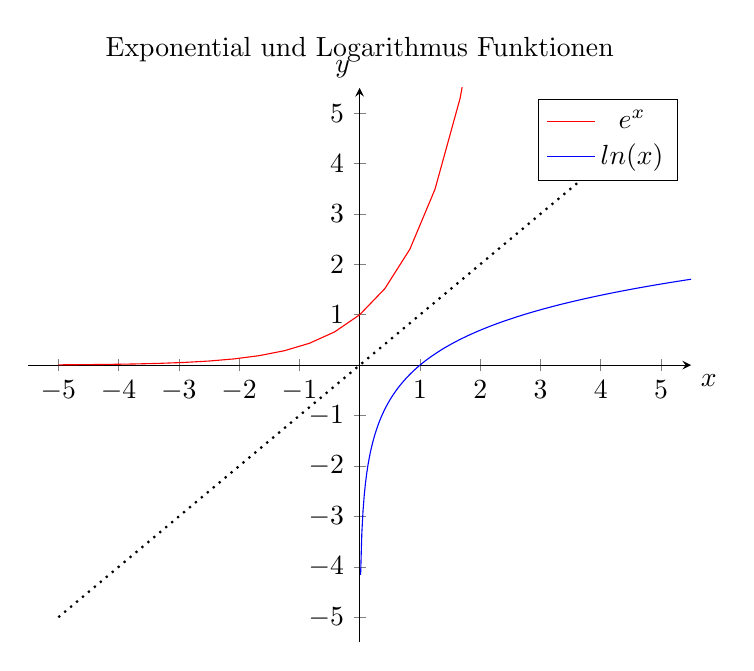
\begin{tikzpicture}
\begin{axis}[
axis x line=center,
  axis y line=center,
  xtick={-5,-4,...,5},
  ytick={-5,-4,...,5},
  xlabel={$x$},
  ylabel={$y$},
  xlabel style={below right},
  ylabel style={above left},
  xmin=-5.5,
  xmax=5.5,
  ymin=-5.5,
  ymax=5.5,
  title = Exponential und Logarithmus Funktionen,
]
\addplot[color=red]{e^x};
\addlegendentry{\(e^x\)}
\addplot [
  blue,domain=1/2^6:10,samples=500
  ] {ln(x)};
\addlegendentry{\(ln(x)\)}
\addplot[color = black, thick, dotted]{x};
\end{axis}
\end{tikzpicture}

\begin{enumerate}

\item Der Graphen der Funktion $f: x\rightarrow \ln x $ enthält man durch \underline{Spiegeln} des Gpraphen von $ c \rightarrow e ^x $ an der Gerade $g: x \rightarrow x$ \underline{(1. Winkelhalbierende)}
\item $\ln x < 0 $ für $ 0 < x < 1 \; ; \; \ln x > 0 $ für $ x> 1$
\item $\ln 1 = 0$
\item 
\begin{align*}
&\Rsh -\infty \quad x \rightarrow 0
\\
\ln x  -----
\\
&\rotatebox[origin=c]{180}{$\Lsh$}+\infty \quad x \rightarrow +\infty
\end{align*}

\item $f(x) = \ln x$ ist \underline{streng monoton steigned} für alle $ x \in D_f$

\item Es gilt \[\frac u {e^x} \rightarrow 0 \text{ für } u \rightarrow +\infty\]
\\
Substitution: \[ u = \ln (x) \Rightarrow e^u = e^{\ln x} = x\]
\\
\[\Rightarrow \frac {\ln x}x \rightarrow 0  \text{ für } x \rightarrow +\infty \text{ (da }e^u \rightarrow +\infty \text{ für } u \rightarrow +\infty)\]
\\
\[ \mathcolorbox{yellow}{\lim_{x \to +\infty} \frac {\ln x }x = 0} \]
\\
\[ \text{also auch } \lim_{x\to _\infty} \frac {\ln x} {p(x)} = 0 \text{ und } \lim_{x \to 0} p(x) \cdot \ln(x) = 0 \text{ falls p(0) } = 0\]
\\
\centerline{(p(x): Polynom)}
\\
$\Rightarrow $ \underline{jedes nichtkonstante Polynom domminiert gegenüber $\ln x $.}

\item Der Graph der Funktion $ f:x \rightarrow \ln x $ ist \underline{rechtsgekrümmt!}

\end{enumerate}

\begin{definition}
Sei $ f: x \rightarrow \ln x \; , \; x \in \mathbb{R}^+$, f ist differenzierbar auf $\mathbb{R}^+$ mit 
\[ f'(x) = (\ln x)' = \frac 1 x\]
\end{definition}

\underline{Beweis: }
\[e^x = y \Rightarrow x = \ln y = \ln e^x\]
\[\Rightarrow (x)' = (\ln e^x)' = [\ln (e^x)]' \cdot (e^x)'\]
\[\Rightarrow 1 = [\ln (e^x)]' \cdot e^x\]
\[\Rightarrow 1 = [\ln y ]' \cdot y \Rightarrow [\ln y ]' = \frac 1 y q.e.d.\]

\subsubsection {Examples:}

1f)
\[f(x) = ln(x-2) - \frac 1 x\]

\[f'(x) = \frac 1 {x-2} + x^{-2}\]

3f)
\[f(x) = ln(x-5) - 2 = 0\]
\[ln(x-5) = 2\]
\[x-5 = e^2\]
\[x = e^2+5\]

5b)
\[f(x) = \ln (x^3)\]
\[f'(x) = \frac {3x^2} {x^3}\]
\[f'(x) = \frac 3 x\] 

10a)
\[f(x) = x - ln(x)\]
\[f'(x) = 1- \frac 1x\]
\[f'(x) = 0 = 1- \frac 1x\]
\[x = 1\]
\[f(1) = 1\]
\[P = [1; 1]\]



\end{document}